\section{Results}\label{sec:results}

  Section 7.2 of the proposal document submitted to BCIT CST BTech outlined all
  tasks that were expected to be achieved as a requirement of this project were
  carried out with a single exception. Part of Task 0.1.8, ``Write simple
  example program as proof-of-concept'' was not. It was felt that the
  justification for developing such a tool was to validate the network
  connectivity and in general the interoperability of this project, but these
  were accomplished using existing tools, namely the command \textt{zmqc} and
  Postman so the time and effort was placed on other aspects. For convenience
  that proposal has been included as a soft copy with this report submission at
  the location \texttt{documents/proposal.pdf}.

  \subsection{Implications}\label{sec:results-implications}

    There are a number of implications that result from the design and
    implementation of this system, some of them were known prior to working on
    the project and some were learned during the course of development. Some
    of these have to do with the complexity of developing and contributing to
    the system going forward, others have to do with requirements placed on
    developing plugins, and finally some have to do with configuration of the
    disparate services and plugins along with the added complexity imposed
    because of the desire to keep all components generic.

    \subsubsection{Development Complexity}

      While some areas of the design were successful and made development
      simpler by employing principles of DRY (don't repeat yourself) others
      were not because of gaps in the design. This can be seen in the REST
      APIs that were developed for each of the separate services, adding and
      editing each of these means making the same changes in the others
      because it was not seen prior to the actual development how having
      filtered APIs in REST calls would be so complicated. So instead of
      being able to chain up to a parent that provides it's own routes each
      needs to provide the same common functionality.

      Another area of complexity that can be seen as a result of this
      implementation is to do with the development of plugins. The services
      were designed to expose a number of different core pieces of
      functionality, for instance the configuration loader, the object
      factories, and the communication components. The implication of having
      developed these in the way that they were is that not enough of the
      overhead is handled by the core API and plugin developers are required
      to do tasks like loading configurations that adhere to the standards of
      the project in order for them to be able to be loaded correctly.

    \subsubsection{Plugin Development}

      One of the learnings of this project, and one of the implications that
      was recognized during the course of implementation, was that while the
      plugin system used made it possible to integrate with any component of
      the systems it also meant that a large amount of work would be offloaded
      to the plugin developer. This was a trade-off because of the amount of
      time that was available during the development phase of the project, in
      order to really make the plugin development a streamlined and simple
      process a redesign of the socket and message queue system would need to
      be done.

      As it is plugins are responsible for a lot more of the message queueing
      and data parsing than they should be. This became most noticeable when
      plugins were developed to generate test data, and consume that data into
      statistics for analyzing traffic. These plugins compress data using the
      ZLib compression which was accomplished in the plugins themselves, this
      was necessary because of the design and structure of the PUB/SUB sockets
      and the data messages that were created to be sent over those wires.

    \subsubsection{Service and Plugin Configuration}

      The last major implication of the design is to do with the configuration
      systems utilized by the services as well as the plugins. A core feature
      of this system is the ability to configure flexible systems for control,
      data acquisition, and data logging, and while this was achieved it was
      at the cost of simplicity of configuration. Each service requires it's
      own configuration, which is as designed, but so do plugins. Configurations
      quickly become complicated to understand if you're not familiar with the
      way that the different networked components wire up to each other.

  \newpage
  \subsection{Research}\label{sec:results-research}

    \subsubsection{Vala}\label{sec:results-research-vala}

      An early consideration of this project was about whether or not selecting
      Vala as the language for development was the right choice. The initial
      motivation for using Vala was primarily because of developer familiarity
      with GObject and GLib, which are core, stable, Linux libraries used for
      the development of several high quality applications. These are developed
      in C so that was an alternative, but Vala is an OOP (Object Oriented
      Programming) language which brings nice syntax for many features that are
      found among those of its type.

      A performance evaluation of three major languages was performed, these
      were C, Vala, and C++. Listings \ref{lst:test-lang-vala},
      \ref{lst:test-lang-c}, and \ref{lst:test-lang-cpp} show the applications
      that were created to perform this test. All three sources were kept as
      similar as possible to achieve a reasonable comparison, however given
      that Vala has GObject/GLib as a base requirement that is where the Vala
      and C examples differ from the C++ one.

      \lstinputlisting[language=c,
                       caption={Vala Test Program},
                       label={lst:test-lang-vala}]
                      {testing/lang-comparison/test.vala}

      \newpage
      \lstinputlisting[language=c,
                       caption={C Test Program},
                       label={lst:test-lang-c}]
                      {testing/lang-comparison/test.c}

      \lstinputlisting[language=cpp,
                       caption={C++ Test Program},
                       label={lst:test-lang-cpp}]
                      {testing/lang-comparison/test.cpp}

      The commands used to compile these examples was:

      \begin{lstlisting}[language=bash]
      # Vala
      valac -X -O2 -X -lm test.vala -o test-vala
      # C
      gcc -O2 -lm `pkg-config --cflags --libs glib-2.0` test.c -o test-c
      # C++
      g++ -O2 -lm test.cpp -o test-cpp
      \end{lstlisting}

      The result of executing these applications three times each and computing
      the averages was:

      \begin{table}[H]
      \centering
      \makebox[0pt][c]{\parbox{1.2\textwidth}{
        \begin{minipage}[b]{0.32\hsize}\centering
          \begin{tabular}{c}
            Vala tests: \\ [0.5ex]
            \midrule
            0.0338 sec \\
            0.0335 sec \\
            0.0332 sec \\
            \midrule
            Average 0.0335 sec \\
          \end{tabular}
        \end{minipage}
        \hfill
        \begin{minipage}[b]{0.32\hsize}\centering
          \begin{tabular}{c}
            C tests: \\ [0.5ex]
            \midrule
            0.0331 sec \\
            0.0335 sec \\
            0.0347 sec \\
            \midrule
            Average 0.0338 sec \\
          \end{tabular}
        \end{minipage}
        \hfill
        \begin{minipage}[b]{0.32\hsize}\centering
          \begin{tabular}{c}
            C++ tests: \\ [0.5ex]
            \midrule
            0.0328 sec \\
            0.0331 sec \\
            0.0340 sec \\
            \midrule
            Average 0.0333 sec \\
          \end{tabular}
        \end{minipage}
      }}
      \end{table}

      From these results it's easy to see that there's no significant
      difference in performance between the languages, this is to be expected
      of Vala because the compiler generates C code itself and spawns the C
      compiler to complete compilation into a binary executable. This meant
      that the decision to go with Vala because of what it brings in terms of
      ease of use to the developer did not come at the cost of performance.

    \newpage
    \subsubsection{ZLib Compression}\label{sec:results-research-zlib}

      The test matrix that was performed is given below in Table
      \ref{tab:zlib-tests}, it was meant to cover conditions that would be
      typical of this kind of system as well as test the upper limits of
      traffic requirements that were defined during the requirements analysis
      phase of the project.

      \begin{table}[H]
        \centering
        \begin{tabular}{c c c c}
          \toprule
          Test \# & Compression & Channel Count & Messages per Second \\ [0.5ex]
          \midrule
           1 & No  & 16  &   1 \\
           2 & No  & 64  &  10 \\
           3 & No  & 128 & 100 \\
           4 & No  & 16  &   1 \\
           5 & No  & 64  &  10 \\
           6 & No  & 128 & 100 \\
           7 & No  & 16  &   1 \\
           8 & No  & 64  &  10 \\
           9 & No  & 128 & 100 \\
          10 & Yes & 16  &   1 \\
          11 & Yes & 64  &  10 \\
          12 & Yes & 128 & 100 \\
          13 & Yes & 16  &   1 \\
          14 & Yes & 64  &  10 \\
          15 & Yes & 128 & 100 \\
          16 & Yes & 16  &   1 \\
          17 & Yes & 64  &  10 \\
          18 & Yes & 128 & 100 \\
          \bottomrule
        \end{tabular}
        \caption{Compression Test Matrix}\label{tab:zlib-tests}
      \end{table}

      For all images given below the blue bars represent uncompressed traffic, and
      the red traffic compressed using standard ZLib compression.

      A comparison of the transfer rates that were measured in all tests with
      and without data compression, across all messaging rates, and all channel
      counts shows no significant improvement in the amount of data transfered
      per unit time. Here we would expect to see a reduction in this number due
      to the constant message rate and expected data reduction due to
      compression.

      \begin{figure}[H]
        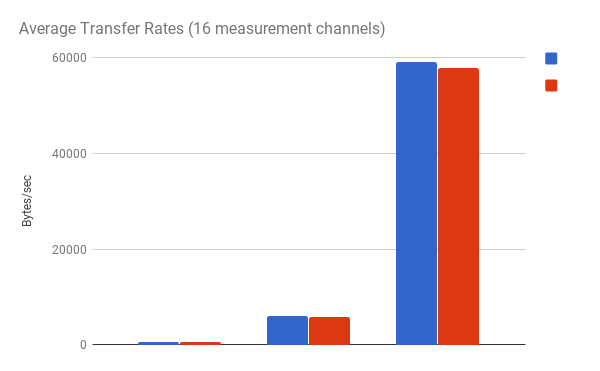
\includegraphics[width=\textwidth]{figures/testing/compression/16mps-avg-tx}
        \caption{Average Data Transfer Rates - 16 Channels}
        \label{fig:zlib-tests-tx-16}
      \end{figure}

      \begin{figure}[H]
        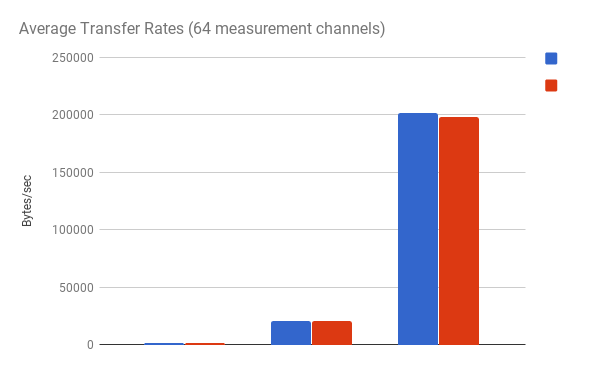
\includegraphics[width=\textwidth]{figures/testing/compression/64mps-avg-tx}
        \caption{Average Data Transfer Rates - 64 Channels}
        \label{fig:zlib-tests-tx-64}
      \end{figure}

      \begin{figure}[H]
        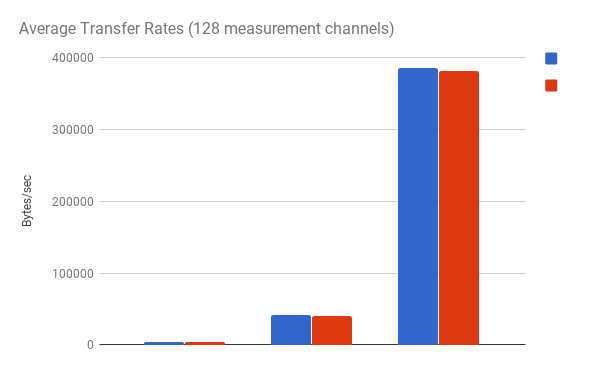
\includegraphics[width=\textwidth]{figures/testing/compression/128mps-avg-tx}
        \caption{Average Data Transfer Rates - 128 Channels}
        \label{fig:zlib-tests-tx-128}
      \end{figure}

      The average transmission times of the message was also compared for data
      measured over the same conditions as was mentioned above. Here it can be
      seen that in the case of the 16 and 64 channel count tests of the the
      transmission times for compressed data is worse by as much as 50\% in
      some cases, but they do scale roughly the same as with the uncompressed
      data. It is worth noting however that the actual differences between test
      data is in all cases less than 100 microseconds which is not exactly
      substantial enough to create concern that the transmission time, or
      communication method, was affected by the data being compressed.

      What is of interest is how in the third case where 128 channels is
      compared the compressed data follows as similar trend, while the
      uncompressed data does not. This is perhaps due to a matching in message
      size to the TCP window size.

      \begin{figure}[H]
        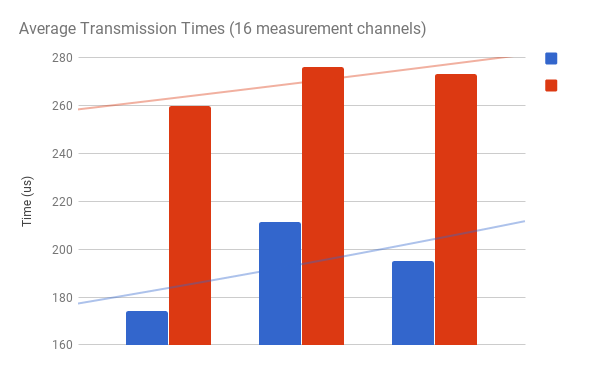
\includegraphics[width=\textwidth]{figures/testing/compression/16mps-avg-msg-time}
        \caption{Average Message Transmission Times - 16 Channels}
        \label{fig:zlib-tests-time-16}
      \end{figure}

      \begin{figure}[H]
        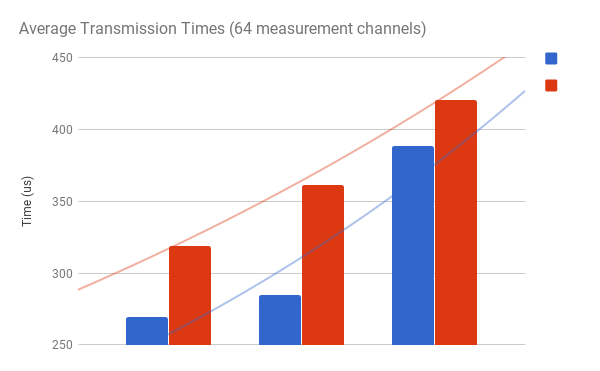
\includegraphics[width=\textwidth]{figures/testing/compression/64mps-avg-msg-time}
        \caption{Average Message Transmission Times - 64 Channels}
        \label{fig:zlib-tests-time-64}
      \end{figure}

      \begin{figure}[H]
        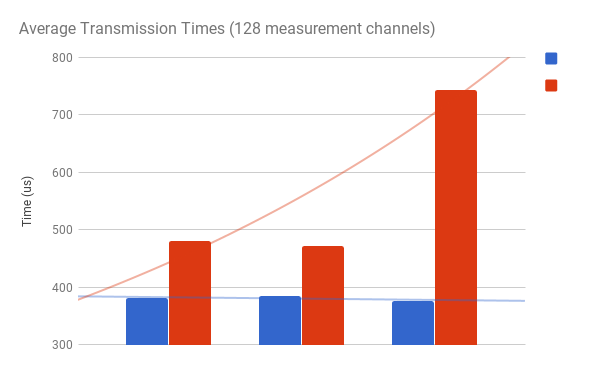
\includegraphics[width=\textwidth]{figures/testing/compression/128mps-avg-msg-time}
        \caption{Average Message Transmission Times - 128 Channels}
        \label{fig:zlib-tests-time-128}
      \end{figure}

      What has been learned by these tests is that there is no significant, or
      insignificant, benefit to compressing the data produced by this projects
      feedback control and data acquisition services.  There was also no
      appreciable overhead imposed by doing so either, so there is still a
      valid case for using compression to transmit data that is measured in
      future systems that come in the form of images, or other large data
      types, especially if communication is to take place between remote
      locations.

  \subsection{Successes}\label{sec:results-successes}

    There were a couple of very important components of this project that
    needed to be carried out successfully, the ability to configure the
    services using a common and consistent format, that each system service
    could load context specific plugins that would perform the heavy lifting
    for data acquisition, data logging, and feedback control, and REST APIs
      which would expose the services and data gathered to just about anything
      that consumes HTTP traffic.

    The configuration systems, which not perfect, do provide the ability to
    construct networked services with a varying number of socket types and
    protocol methods at runtime without writing any additional code, and
    without even needing to compile any code. This may exist elsewhere in
    similar forms, but not that this author has been able to find so the
    ability to perform this kind of flexible networking is seen as a project
    accomplishment.

    Plugin systems are crucial to this system, the project was to define a
    framework for application development that use a variety of different kinds
    of data acquisition hardware devices, data logging backends, and feedback
    control schemes. This was achieved by making each service load plugins and
    expose parts of their data models to those plugins so that the actual work
    could be done without knowing what the hardware is or need to do for the
    development of the services.

    REST service routers open up a lot of possibilities including websites that
    pull data using standard web requests, this should make application
    development much easier long term for any project that needs to pull data
    from a data log, retrieve a measured value, or perform complicated control
    systems without having to actual modify any of the systems that perform
    those tasks.

  \subsection{Failures}\label{sec:results-failures}

    The idea of being able to have services and plugins be configurable from a
    variety of input types was an interesting one as it would allow for the
    developer of such things to make choices about how they wanted to configure
    their component, but it created added complexity where it wasn't necessary.
    Using a single format, ideally JSON, would have simplified development and
    much of the development could have been focussed on systems that were more
    crucial to execution.

    Configuration exceptions are too restrictive and not always handled
    correctly so the service will fail if there are issues with what's been
    provided, such as an object that the service does not have a factory to
    construct. This is not a show stopper due to the fact that the editor
    shouldn't need to add objects that aren't available in the libraries, but
    it should skip them gracefully with the addition of a warning message and
    allow the rest of the data model to be constructed successfully.
